\chapter{Onderzoeksplan}\label{ch:onderzoekPlan}

In het vorige hoofdstuk is de opdracht voor dit onderzoek duidelijk uitgeschreven. In dit hoofdstuk wordt uitgewijd over hoe deze opdracht wordt uitgevoerd, welke bronnen er gebruikt worden en hoe het onderzoek gedaan zal worden. Het resultaat is het een onderzoeksplan voor een onderzoek naar analyses op kwetsbaarheden op externe bibliotheken(SOUP) binnen EagleScience. Als leidraad voor dit hoofdstuk is gekozen voor \cite{JanLeen2017}

\section{Aanleiding}\label{sec:OP_aanleiding}
EagleScience heeft de ambitie om te groeien in zowel het aantal projecten dat het aanneemt als in het aantal medewerkers. Daarnaast is het bezig met het integreren van het software lifecycle management paradigma in het kwaliteitssysteem om zo een gerichte-, transparante en traceerbare aanpak te hebben over de kwaliteit en daarmee de veiligheid van de te leveren software. Vooral de groei in projecten heeft geleid tot deze opdracht. Het feit dat EagleScience aanbied om de door ons ontwikkelde applicaties te hosten voor de klant zullen deze in de komende tijd ook aannemen. Hierdoor neemt de druk op het DevOps team binnen EagleScience toe. Om deze druk te verminderen wordt er gezocht naar manieren om taken die veel voorkomen en bijdragen aan de kwaliteit te automatiseren om op die manier een traceerbare en transparante aanpak te hebben.

\section{Probleemanalyse}\label{sec:probleemanalyse}
[NOTE: WIE< WAT< WAAR< WAAROM< WANNEER< WAARDOOR]
EagleScience doet veel om veilige applicaties te leveren voor haar klanten. Tijdens het ontwikkelproces wordt er door de ontwikkelaars continue afgewogen welke maatregelen, in architectuur en/of code, moeten worden genomen applicaties veilig op te leveren. Deze afwegingen zijn onderdeel van het ontwerpproces en worden door de klant gezien als declarabele uren en zijn ook bereid voor deze werkzaamheden te betalen. Op het moment dat een project "klaar" is over gaat van ontwikkeling naar hosting. Wordt er onderhoud gedaan volgens afspraken in de SLA. In diezelfde SLA wordt niet altijd ruimte opgenomen voor het analyseren van de applicatie op kwetsbaarheden. Vaak komt dit doordat de klant er geen budget voor heeft, of het niet belangrijk vindt. Gezien EagleScience alleen een advies kan uitbrengen over support en de klant de eindbeslissing heeft. Maar omdat EagleScience wel zo "veel mogelijk" wil garanderen dat de software die gehost wordt veilig is dient de applicatie in hosting periodiek geannalyseerd worden op kwetsbaarhebeb. Op dit moment is dit een tijdrovend handmatig process waarbij een teamlid ongeveer 8 tot 12 bezig om iedere dependency te bekijken of er updates zijn en welke mogelijke kwetsbaarhden er zijn. Door de groei die EagleScience binnenkort wil maken is er de wens om bovestaand proces te automatiseren.

Er moet dus een methode worden ontwikkeld die het mogelijk maakt om geautomatiseerd en periodiek een analyse te doen op dependencies die gedeclareerd zijn in het project. De analyses moeten inzichtelijk maken welke componenten er genanalyseerd zijn inclusief versie nummer. En of er kwetsbaarheden zijn gevonden in deze bibliotheken. De methode moet voor alle platformen(Docker, Programmeertalen, Databases etc.) dezelfde resultaten geven.

Door de analyses te automatiseren wordt beoogd dat er minder tijd wordt besteed aan de analyse. Deze tijd kan dan worden besteed door de ontwikkelaar aan taken die declarabel zijn en voor beide partijen winstgevend zijn.


%Probleem stelling
Samengevat is het probleem als volgt: "Handmatig SOUP-analyses doen kost tijd die niet declarabel zijn. Om deze reden is de wens dat er een geautomatiseerde oplossing komt die periodiek de projecten die in ontwikkeling zijn en/of gehost worden door EagleScience geanalyseerd wordt op kwetsbaarheden in gebruikte externe bibliotheken. Door deze automatische oplossing wordt ingeschat dat de (niet declarabele) uren die normaal gebruikt worden voor analyseren van de projecten gebruikt kunnen worden voor andere wel declarabale uren.

De huidige handmatig uitgevoerde SOUP-analyses zijn tijdrovend waardoor ontwikkelaars andere taken moeten laten vallen. Daarnaast wordt de analyse niet frequent genoeg gedaan en vaak enkel op inplanbare momenten. De probleemstelling luidt: "Ontwikkel een methode die automatisch en periodiek een SOUP-analyse doet op de projecten die EagleScience in haar beheer heeft".

De probleemstelling geeft de volgende Centrale vraag: "Welke methode is het meest geschikt voor het geautomatiseerd en periodiek uitvoeren van een SOUP analyse voor alle in beheer zijnde projecten binnen EagleScience?


\section{Doelstellingen}\label{sec:doelstellingen}
Het doel van dit onderzoek is het ontwikkelen van een methode om een SOUP-analyse te doen binnen de dev-stack van EagleScience. Hierbij moet rekening gehouden worden met de in de opdracht gegeven criteria, waarvan de belangrijkste is dat er zo min mogelijk impact moet zijn op de huidige werkwijze. Aan het einde van het onderzoek moet dus een methode worden gepresenteerd die vervolgens bewezen kan worden middels een implementantie van een  analyse op de twee meest gebruikte technologiën binnen EagleScience. De implementatie wordt dan ook in deel \ref{prt:Implementatie} beschreven.



\section{Stakeholdersanalyse}\label{sec:stakeholdersanalyse}
Om te kijken naar het draagvlak voor dit onderzoek dient er een stakeholders analyse gedaan te worden. Op deze manier moet het duidelijk worden wie de stakeholders zijn en welke belangen zei hebben bij het doen van een onderzoek naar een geautomatiseerde SOUP-Analyse en de resultaten hiervan.

\subsection{Dagelijks bestuur (intern)}\label{subsec:dagelijks-bestuur-(intern)1}
Het dagelijks bestuur ziet vooral voordelen in het op een overzichtelijke manier verkrijgen van inzichten in kwetsbaarheden. Zij beogen dat ze hierdoor beter kunnen aansturen in het gebruik van bibliotheken en/of andere technologiëen. Ondanks dat de ontwikkeling van de beoogde nieuwe module vooral geld zal kosten, is de huidige manier van werken ook niet kosten-effectief. Daarnaast voorziet de CTO dat de nieuwe module tijdswinst zal opleveren waardoor de time-to-market voor andere projecten hoger kan komen te liggen en er dus op langer termijn meer verdiend kan worden.

\subsection{Projectmanagers (intern)}\label{subsec:projectmanagers-(intern)1}
Project managers krijgen op dit moment een update over de staat van kwetsbaarheden op het moment dat een analyse gedaan is. Veelal na een deploy of als er naar gevraagt is. De nieuwe module zal ze echter de mogelijkheid bieden om up-to-date informatie on-demand te verkrijgen.
De tijdsinvestering die nodig is van ontwikkelaars voor de ontwikkeling van de module weegt volgens hen op tegen de voordelen die de module in de toekomst kan brengen.

\subsection{Ontwikkelteam (intern)}\label{subsec:ontwikkelteam-(intern)1}
Het handmatig testen van kwetsbaarheden werd tot op heden gedaan door het ontwikkelteam. Dit is een tijdrovende taak, welke ten koste gaat aan de ontwikkeling van software voor klanten. Het ontwikkelteam heeft daarrom direct baat bij de ontwikkeling van de beoogte module en wil daarom graag hieraan meedenken en meewerken.

\subsection{Klant (extern)}\label{subsec:klant-(extern)1}
De enige externe stakeholder is de klant. Dit is tevens een passieve stakeholder gezien zij niet direct betrokken zijn bij de ontwikkeling van de module, maar wel baat hebben bij de uitkomst hiervan, namelijk in de vorm van veiligere en betrouwbaardere software tegen potentieel lagere kosten.

\subsection{Stakeholder analyse}\label{subsec:stakeholder-analyse1}
\begin{figure}[H]
    \myfloatalign
    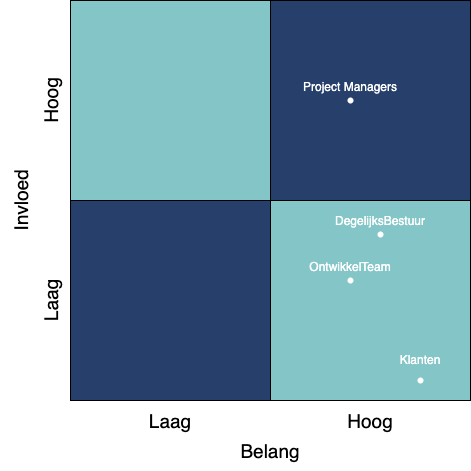
\includegraphics[width=10cm]{gfx/stakeholderanalyse}
    \caption{StakeHolders Analyse}
    \label{fig:StakeholderAnalyse1}
\end{figure}
[NOTE]Figuur stakeholder analyse nog aanpassen.
Zoals te zien is in figuur~\ref{fig:StakeholderAnalyse1} zijn de projectmanager, het ontwikkelteam en de klanten het meest gebaad bij een nieuwe module voor de analyse van kwetsbaarheden.
Door deze analyse worden alleen de requirements meegenomen die intern zijn opgenomen.


\section{Theoretisch kader}\label{sec:theoretisch-kader}

Het theoretisch kader waarmee gewerkt wordt bestaat uit twee hoofddelen. Het eerste hoofddeel is de werkwijze van EagleScience en de gebruikte technologiëen. De volgende bronnen zullen bij het onderzoek worden gebruikt:
\begin{itemize}
    \item \textbf{151030 F04B Proces Flow Chart ES\_V1.0\_TN.pdf} een document dat de workflow beschrijft die binnen EagleScience gehanteerd wordt.
    \item \textbf{200121\_Policy Manual\_ES\_V6 signed.pdf} ISO handboek waarin de bedrijfsvoering binnen EagleScience wordt beschreven.
\end{itemize}
Deze documenten vormen de basis over de werkwijze van EagleScience en zal als input gelden voor het ontwerp dat plaats gaat vinden na het onderzoek.

Het tweede hoofddeel is de theorie over externe bibliotheken. Het richt zich op het gebruik hiervan, de potentiële gevaren en methoden om deze bibliotheken te analyseren. Als ingangspunt is de OWASP Top-10 gekozen omdat de inhoud van dit document binnen EagleScience geldt als aandachtspunten voor het ontwikkelen van veilige software. De basis voor dit onderzoek wordt beschreven in punt "A06:2021-Vulnerable and Outdated Components". Hier wordt beschreven welke gevaren er potentieel dreigen als op dit punt niets gedaan wordt. Andere bronnen zijn:
\begin{itemize}
    \item \textbf{OWASP top 10 (https://owasp.org/Top10/)} hierin staan de belangrijkste aandachtspunten die door een onderzoek vanuit de OWASP aan het licht zijn gekomen. Op A06:2021 staat een melding over kwetsbaarheden en outdated Components.
    \item \textbf{Detail pagina OWASP A06:2021(https://owasp.org/Top10/A06_2021-Vulnerable_and_Outdated_Components/)} OP deze pagina zijn details te vinden over item A06:2021 waaronder een beschrijving, Hoe het te voorkomen is en een aantal voorbeeld scenario's waarbij een aanval wordt geillustreerd.
    \item \textbf{OWASP dependency-check (https://owasp.org/www-project-dependency-check/)} Pagina over het project binnen de OWASP voor het analyseren van componenten in Applicaties
    \item \textbf{Justifying the use of software of uncertain pedigree (SOUP) in safety-related applications} P.G.\ Bishop, R.E.\ Bloomfield and P.K.D.\  Froome for Adelard 2001. Hoewel dit document verouderd lijkt staat er wel degelijk interessante informatie over waarom je SOUP zou gebruiken en hoe je de risico's kan verminderen.
    \item \textbf{Backstabber’s Knife Collection: A Review of Open Source Software Supply Chain Attacks} Marc Ohm, Henrik Plate, Arnold Sykosch, and Michael Meier: 2020: Dit artikel bevat informatie over een mogelijke vorm van aanvallen die middels SOUP uitgevoerd zouden kunnen worden. Daarnaast geeft het artikel inzicht in hoe de onderzoekers packages voor NPM, Python, en Ruby hebben onderzocht.
\end{itemize}
Het laatste hoofddeel bestaat uit de resultaten van de bovengenoemde onderdelen waarmee een voor EagleScience geschikte methode wordt gevonden. Naast de resultaten van de twee voorgaande hoofddelen worden de volgende bronnen geraadpleegd als leidraad voor het ontwerp:

\newpage %TODO: Echt nodig?
\section{Conceptueel model}\label{sec:conceptueel-model}
Om de relevantie en relatie van de verschillende onderzoeken te waarborgen is het volgende conceptueel model opgesteld.
\begin{figure}[H]
    \centering
    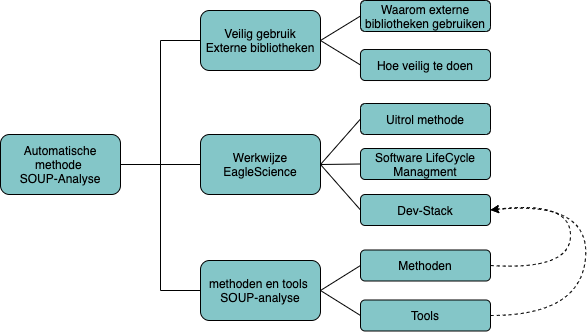
\includegraphics[width=12cm]{gfx/Conceptueel Model}
    \caption{Conceptueel Model}
    \label{fig:ConceptueelModel}
\end{figure}

In figuur~\ref{fig:ConceptueelModel} is het conceptueel model opgenomen dat voor deze opdracht is opgesteld. Dit model maakt de samenhang van de verschillende begrippen duidelijk.

Het kernbegrip is "Automatische methode SOUP analyse" en staat voor de eind conclusie die het onderzoek moet opleveren in de zin van een conclussie over tools en een methode die gebruikt kunnen worden in het ontwerp van de module. Om tot deze conclussie te komen zijn er vier begrippen die ieders een eigen domein binnen de probleemstelling belichten. Zo zal "werkwijze EagleScience" de manier van werken binnen Eaglescience belichten als ook de manier van uitrollen en de dev-stack die gebruikt gaat worden. Ook komt hier de Software Lifecycle Managment aan bod gezien dit één van de aanleidingen voor de opdracht. Het theoretische deel van het onderzoek wordt onderzocht in "veilig gebruik externe bibliotheken" waarin wordt gekeken waarom er bibliotheken van buitenaf worden gebruikt en wat de potentiële gevaren zijn die dit met zich meebrengt. Het begrip methoden en tools zal ingaan op de beschikbare tools die gebruikt kunnen worden om een analyse te doen. Met deze tools wordt een methode onderzocht die het mogelijk maakt met de constraints die EagleScience heeft om een SOUP analyse te doen. Met als resultaaat een theoretische methode die als input kan gelden voor het ontwerp voor de nieuwe module die in de opdracht staat beschreven. Deze nieuwe module dient in de EagleScience Portal opgenomen te worden en om die reden is het begrip "Huidig architctuur EagleScience Portal" waarin wordt onderzocht hoe de portal ontworpen is en welke dev-stack er is gebruikt.

\section{Deelvragen}\label{sec:deelvragen}
Aan de hand van het theoretisch kader, conceptueel model en de doelstellingen zijn er de volgende deelvragen voor dit onderzoek opgesteld:
\textbf{Dev-stack binnen Eaglescience}
\begin{itemize}
    \item Hoe wordt binnen EagleScience het software lifecycle management paradigma ingevoerd?
    \item Welk proces wordt er binnen EagleScience gebruikt om software te ontwikkelen en hoe resulteert dit is een dagelijkse werkwijze?
    \item Wat zijn de meest gebruikte ontwikkeltalen en frameworks die binnen EagleScience worden toegepast?
    \item Welke tooling wordt er gebruikt binnen EagleScience? [NOTE relevant?]
    \item Hoe wordt er binnen EagleScience software uitgerold?
\end{itemize}
\textbf{Theorie over SOUP}
\begin{itemize}
    \item Wat is veilige software?
    \item Wat is SOUP?
    \item Wat dragen externe bibliotheken en dus ook potentieel SOUP bij aan de ontwikkeling van software?
    \item Wat zijn de gevaren van het gebruik van SOUP?
    \item Wordt er ergens bijgehouden of een dependency/component een kwetsbaarheid bevat?
    \item Wat relateert SOUP tot software veiligheid binnen EagleScience?
    \item Welke methodes en tools zijn er beschikbaar voor SOUP analyse?
\end{itemize}
\textbf{Methodes om een SOUP analyse te doen binnen de Dev-stack van EagleScience}
\begin{itemize}
    \item Welke tools bestaan er om dependency informatie uit een sbt en npm project te halen?
    \item Hoe zijn de tools in te zetten in de huidige projecten?
    \item Welke output wordt er verkregen van de tools?
    \item Welke manieren zijn er om uit de huidige pipeline informatie over de deploy te halen?
    \item Wat zijn hier de voor-, en nadelen van?
\end{itemize}


\section{Onderzoeksontwerp}\label{sec:onderzoeksontwerp}
Gezien de grote hoeveelheid deelvragen die benoemd zijn op basis van de onderzoeksvraag en het conceptueel model is het verstandig om het onderzoek in kleinere deelonderzoeken te verdelen. Door het op te delen in deelonderzoeken kan het kader beter worden vastgesteld en zal er minder snel "teveel" worden onderzocht. De deelonderzoeken zullen op de volgende manier worden opgesplitst:
\begin{enumerate}
    \item \textbf{Werkwijze en dev-stack EagleScience} Dit onderzoek moet inzicht geven in de dagelijkse manier van werken binnen EagleScience en de daarbij gebruikte dev-stack. Het doel is inzicht verkrijgen in hoe EagleScience applicaties ontwikkeld, hoe deze uitgerold worden en hoe er op dit moment SOUP analyses worden uitgevoerd.
    \item \textbf{Theorie SOUP analyses} Om een methode te kunnen ontwikkelen is er een theoretische basis nodig. Dit onderzoek geeft inzicht in de theoretische basis en het belang van SOUP analyses. Daarnaast wordt er uitgezocht hoe er het beste een analyse gedaan kan worden.
    \item \textbf{Methode voor SOUP analyse binnen EagleScience} Door inzichten uit voorgaande onderzoeken te combineren en nieuwe kennis toe te voegen is er een ontwerp voor een implementatie die aan de opdracht voldoet.
\end{enumerate}

\subsection{strategie}\label{subsec:opstrategie}
Om de drie onderzoeken die hierboven beschreven zijn goed uit te kunnen voeren zijn er de volgende strategieen bedacht die ervoor zorgen dat er een betrouwbaar resultaat is waar verder mee gewerkt kan worden.
Voor het onderzoek binnen de huidige situatie binnen EagleScience wordt interne documentatie geraadpleegd aangevuld met vraag gesprekken met collega's die met het onderwerp te maken hebben. Deze gespreken zullen worden gehouden in delen gezien de manier waarop er binnen EagleScience gewerkt wordt. (heeft te maken met het aantal niet declarabele uren die ieder persoon wel of niet heeft). Het onderzoek naar de theorie van SOUP analyses wordt uitgevoerd middels een deskresearch waarbij in literatuur gezocht wordt naar methoden om de analyse te doen. Daarnaast wordt er een selectie gemaakt in tools die al ontwikkeld zijn die bruikbaar zijn voor het einddoel van de opdracht. In het laatste onderzoek wordt gekeken naar een method die past bij de huidige manier van werken binnen eaglescience, en de tools die gevonden zijn. Ook wordt er een ontwerp gemaakt hoe de methode eruit komt te zien er welke data dit oplevert waarna er een module ontwikkeld kan worden die deze data inzichtelijk maakt voor de stakeholders.

\section{planning}\label{sec:planning}
Om tijdig tot resultaten te komen is de volgende planning opgesteld.

\subsection{Requirements analyse \textbf{september 2021}}\label{subsec:requirements-analyse}
Na het ontvangen van de opdracht dient er onderzocht te worden of er naast de eisen die door de CTO in de opdracht zijn gezet nog andere eisen zijn binnen EagleScience. Hiervoor zal er onderzocht worden welke betrokkenen er zijn en welke belangen en wensen zij hebben. Na het houden van interviews zullen alle wensen tegen elkaar worden afgewogen. Dit zal leiden tot een document waarin alle belangrijke requirements worden geprioriteerd volgens de MoSCoW\-methode.

\textbf{Methode:} Intake gesprek met opdrachtgever, interviews met betrokkenen, enquete voor ontwikkelaars.

\textbf{Resultaat:} Applicatie requirements document.

\subsection{Vooronderzoek \textbf{september 2021 - oktober 2021 }}\label{subsec:onderzoek}
Om de requirements om te kunnen zetten naar een ontwerp zal er onderzoek gedaan worden naar de huidige manier van ontwikkelen en compileren van de software. Een onderzoek naar begrippen binnen het domein SOUP is een voorwaarde om vervolgens onderzoek te kunnen doen naar methodes om analyses te kunnen doen op software die EagleScience maakt ten opzichte van SOUP. De resultaten van het vooronderzoek zullen worden gebruikt als input.
Om meer kennis en verdieping te krijgen in de materie rondom de nieuwe module zullen er een aantal onderzoeken worden uitgevoerd.


Er is onderzoek nodig naar de volgende onderwerpen:
\begin{itemize}
    \item \textbf{Architectuur binnen EagleScience} Werkwijze en ontwikkel stack van EagleScience met daarin specifiek onderzocht hoe er omgegaan wordt met het voorkomen van onveiligheden in de geleverde software
    \item \textbf{Externe bibliotheken gebruik en het gevaar} Onderzoek naar waarom er externe bibliotheken worden gebruikt en het gevaar hiervan.
    \item \textbf{Soup Analyse} Door te kijken naar de kwetsbaarheden in de externe bibliotheken kan er beter worden nagegaan of er kwetsbaarheden in de software zitten. Dit onderzoek zal in gaan op het bestaan van methodes om SOUP analyses te doen. En een mogelijkheid om dit (deels) geautomatiseerde te doen.
\end{itemize}

\textbf{Methode:} Bureau onderzoek, interviews met specialisten, meedoen aan en/of terugkijken van conferenties

\textbf{Resultaat:} Inzicht in het begrip SOUP en software veiligheid als ook een idee voor een mogelijke implementatie van de oplossing die voor EagleScience de beste is zonder veel impact op de huidige manier van werken te hebben.

\subsection{Initieel ontwerp \textbf{oktober 2021 - november 2021 }}\label{subsec:initieel-ontwerp}
Er zal een ontwerp worden gemaakt waarin vast gelegd is welke requirements er beslist in de module moeten zitten en de uitwerking van deze. Evenals een ontwerp van de architectuur en het datamodel. Naast de module zal er ook een ontwerp gemaakt worden voor een ontwikkel/test omgeving om de module continue te kunnen testen zonder dat dit de huidige buildstraat beinvloed. Dit laatste is van belang om zo min mogelijk storingen te veroorzaken in de dagelijkse gang van zaken bij al lopende projecten. Het eerste ontwerp zal als leidraad dienen voor de implementatie waarin afgeweken kan worden als dit nodig blijkt tijdens de implementatie sprints.

\textbf{Methode:} Overleggen met ontwikkelaars, huidige omgeving onderzoeken op mogelijkheden en architectuur.
\textit{wellicht nog toevoegen als resultaten: blokdiagram van oplossing/architectuur; sequence diagram om te komen van analyse tot rapportage (er is een handig tooltje om deze diagrammen te tekenen: https://bramp.github.io/js-sequence-diagrams/)}
\textbf{Resultaat:} Eerste ontwerp in de vorm van een datamodel, blokdiagram van architectuur voor de oplossing, als ook een sequence diagram om van analyse tot rapportage te komen.

\textit{4.4: Gebruik hier of de template ontwikkel omgeving voor (aparte branch/taak); of de portal ontwikkelomgeving
4.4: Voeg rij resultaat toe: klaar voor review of gereviewde}

\subsection{Implementatie en Testen \textbf{november 2021 - januari 2022 }}\label{subsec:implementatie-en-testen}
Om te kunnen beginnen aan de implementatie is er een ontwikkel/ test omgeving nodig die het mogelijk maakt om zonder invloed op de dagelijkse werkzaamheden van EagleScience een module te kunnen ontwikkelen. Deze zal eerst worden opgezet. Als test projecten zullen snapshots worden gebruikt van de daadwerkelijke projecten dit om een zo accuraat mogelijke test omgeving te hebben. Zoals in de opdracht beschreven dient de nieuwe module een onderdeel te zijn van de bestaande portal. Er zal dan ook direct samen worden gewerkt met het team die daar op het moment mee aan het ontwikkelen is. Tijdens de implementatie zal er ook worden gedocumenteerd wordt hoe de module werkt en welke procedures hier in worden gevolgd. Dit document biedt ontwikkelaars de mogelijkheid om dit door te nemen als on-boarding en referentie.

\textbf{Methode:} Agile scrum sprints met iedere 2 weken een oplevermoment en demo als ook een reflectie op de sprint.
\textbf{Resultaat:} Werkende en geteste applicatie die klaar is om uitgerold te worden.

\subsection{Uitrollen en documentatie \textbf{januari 2022 - februari 2022 }}\label{subsec:uitrollen-en-documentatie}
Nadat de implementatie van de meest kritische requirements is afgerond zal er worden begonnen met het uitrollen van de module en het testen door een geselecteerde groep gebruikers. De feedback wordt bekeken en meegenomen in de evaluatie. Mocht het nodig zijn dan zal er accuut actie worden ondernomen om deze wijzigingen aan te passen. Mochten er wensen zijn die kunnen wachten dan zal er worden overwogen om deze mee te nemen in de volgende iteratie van het project. (de verwachting is dat de module die hier beschreven wordt verder zal worden uitgebreid met de diverse mogelijkheden om betere en veiligere software te ontwikkelen.) Daarnaast zal ook de documentatie verder worden afgerond.
\textbf{Methode:} Interviews met stakeholders met een analyse over de nieuwe requirements.

\textbf{Resultaat:} Uitgerolde en gedocumenteerde applicatie
